\chapter{Implementation}

A part of this work is an experimental implementation of our proposed algorithm. Besides our approach, we have also implementened the algorithm proposed in \cite{RepAndConsistentAnswer}, to be able to compare it with our algorithm. Our algorithm has been implemented in the Java language, version 6.0 as a part of the schema inference framework for XML called jInfer \cite{jinfer}.

\section{jInfer Framework}

jInfer framework was developed as a Software Project at the Faculty of Mathematics and Physics, Charles University at Prague. The framework is based on the NetBeans platform and is mainly used for XML schema inference. Although our proposed algorithm is not dealing with schema inference, jInfer is designed to be extensible and is suitable for incorporation of our algorithm.

The whole process of repairing inconsistent XML data is divided three steps (illustrated in Fig. \ref{repairProcess}):

\begin{enumerate}
	\item Import of input data (XML, functional dependencies, weights) into an internal representation - \emph{Initial Model}.
    \item Repairing of \emph{Initial Model} with optional help of user interaction.
    \item Export back the repaired data into XML format.
\end{enumerate}

\begin{figure}[H]
    \centering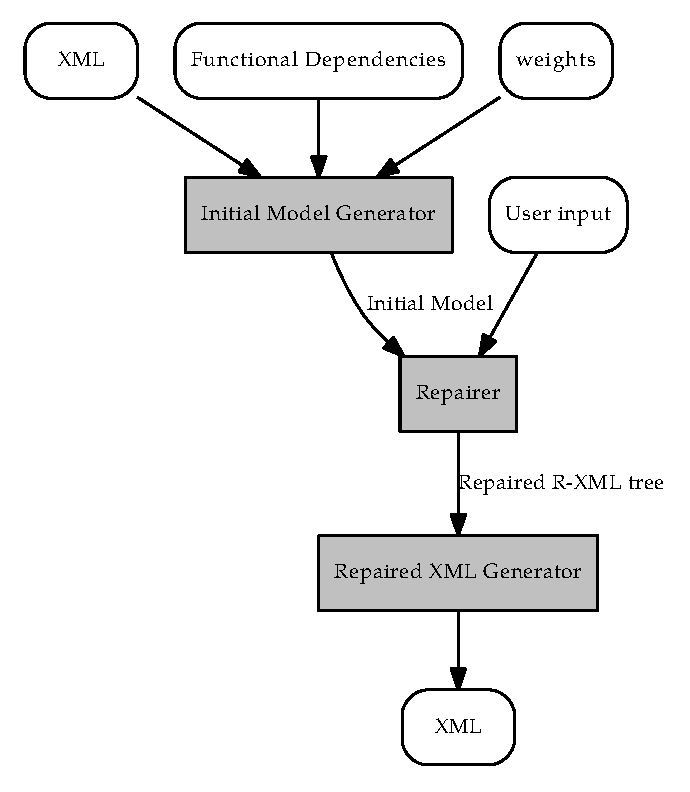
\includegraphics[width=0.6\textwidth]{repair_process}
    \caption{High-level view of the repair process}
    \label{repairProcess}
\end{figure}

\section{Architecture}

The main part of our algorithm is implemented as the \texttt{FDRepairer} module of the jInfer framework. The core package of the module is \texttt{cz.cuni.mff.\discretionary{}{}{}ksi.jinfer.functionalDependencies} and contains classes representing base object important for repairing (Tuple, RW-XML tree, Path etc.). This package is further divided into the following subpackages:

\begin{description}
	\item[fd] contains data structure of functional dependencies used as an input to the algorithm.
    \item [interfaces] contains Java interfaces necessery for integration in the jInfer framework.
    \item [modelGenerator] contains classes responsible for creating data structures from loaded input files.
    \item [newRepairer] contains class \texttt{NewRepairerImpl}, the class that implements our proposed algorithm. Also it contains other data structures introduced in our approach
    \item [properties] contains classes reponsible for showing properties of this extension in the jInfer.
    \item [repairer] contains classes implementing the original algorithm from \cite{RepAndConsistentAnswer}.
    \item [weights] contains data structure for node weights used as an input to the algorithm.
\end{description}

\subsection{Input Files Processing}

Files that can be added as an input to our algorithm are of three types. The XML data, file containing functional dependencies and file containing weights. First, the XML is processed with build-in Java DOM parster. Files with FDs and weights both contain XML data with specific structure defined as XML Schema in Fig. \ref{fdschema} and \ref{weightschema} and are both processed with JAXB \cite{JAXB}.


\section{Restriction of Implementation}

The \texttt{FDRepairer} module of the jInfer framework is an implementation of our proposed algorithm presented in Chapter \ref{kap4}. However, one part of the algorithm have not been implemented yet, namely the intersection of repair candidates with existing repair group.

\section{Building and Executing}

For building jInfer with \texttt{FDRepairer} from sources, please refer to the tutorial at \url{http://jinfer.sourceforge.net/building_jinfer.html}. To execute jInfer, install plugins from enclosed CD or built from sources into NetBeans.

Appendix C contains a simple user guide with screenshots about how to use \texttt{FDRepairer}.
